\begin{figure}[t]
    % First row
    \centering
    \begin{subfigure}{0.46\textwidth}
        \centering
        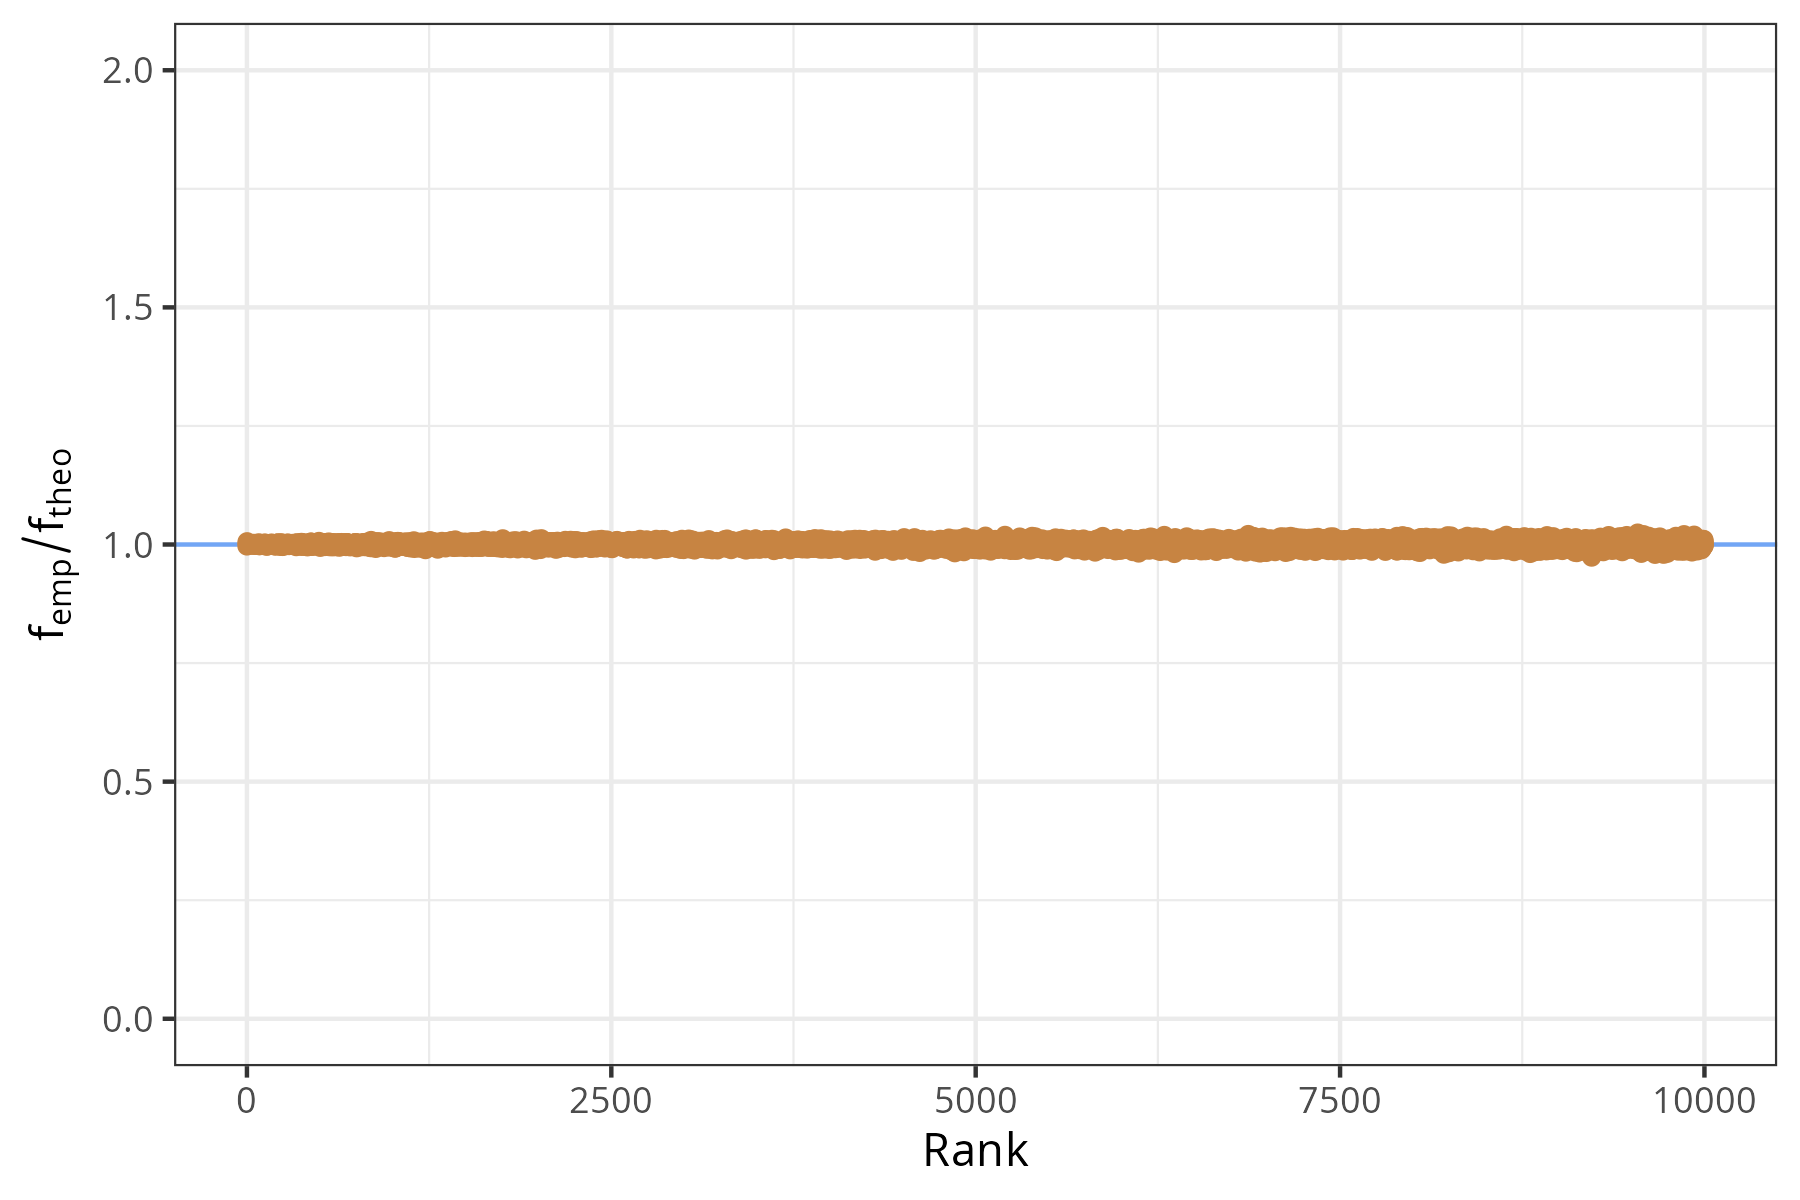
\includegraphics[width=\textwidth]{figures/ratio/apache.png}
        \caption{Rejection inversion}
    \end{subfigure}
    \hfill
    \begin{subfigure}{0.46\textwidth}
        \centering
        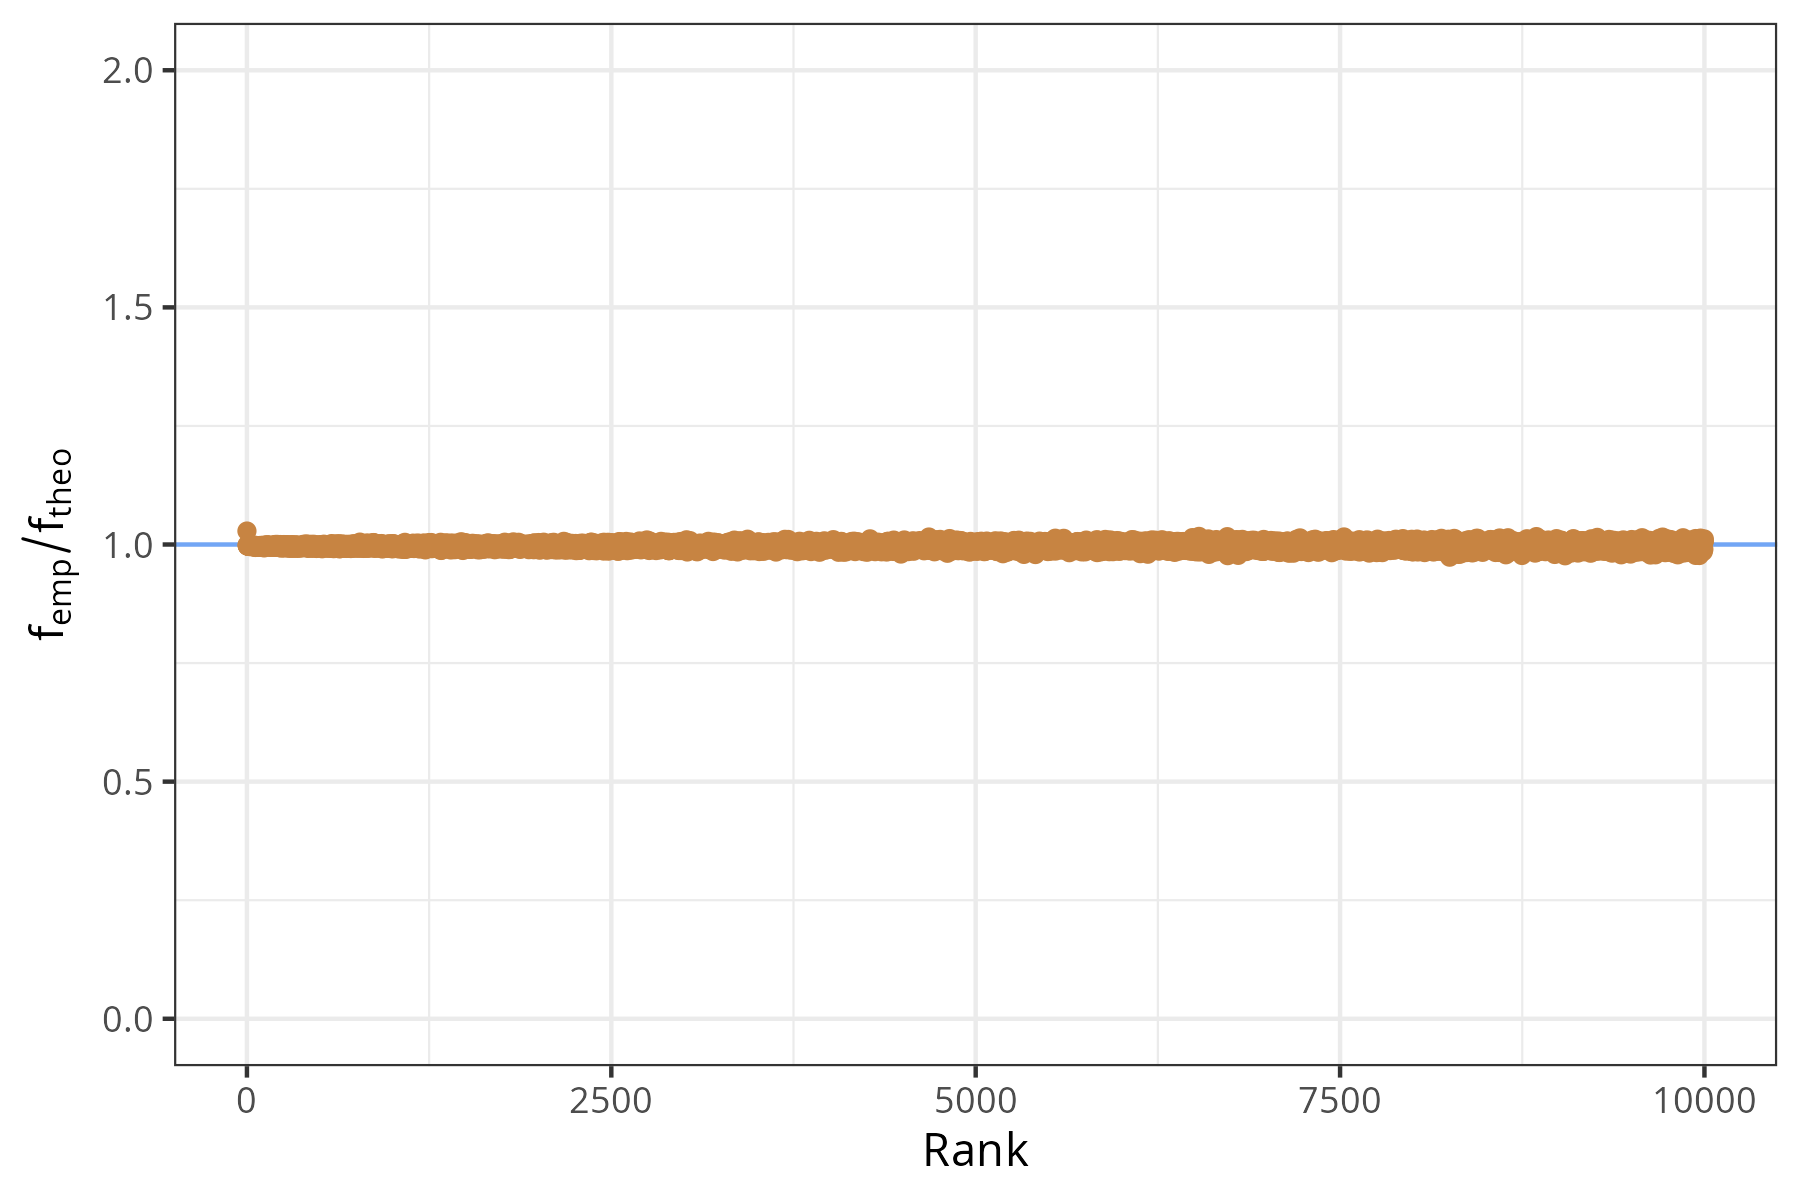
\includegraphics[width=\textwidth]{figures/ratio/ycsb.png}
        \caption{YCSB}
    \end{subfigure}
    
    \vspace{1em} % Space between rows
    
    % Second row
    \begin{subfigure}{0.46\textwidth}
        \centering
        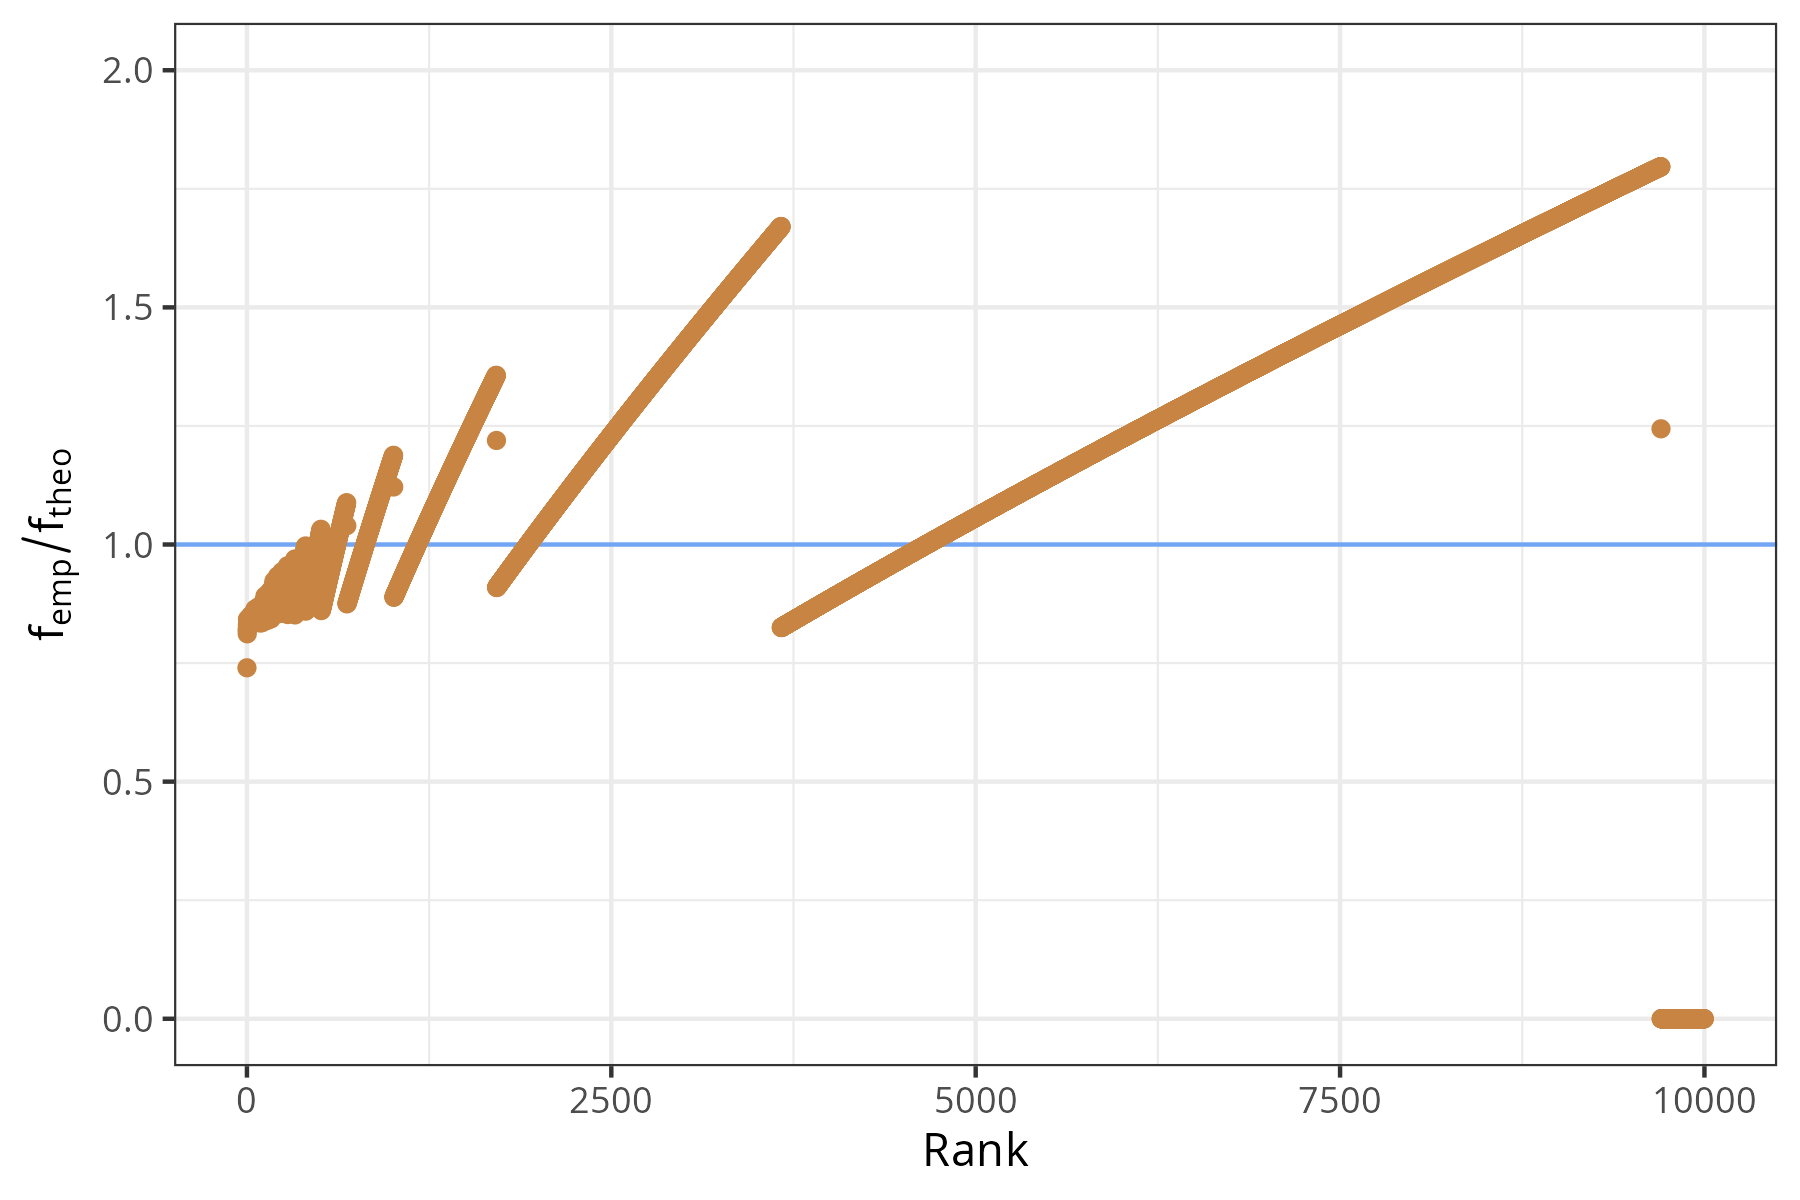
\includegraphics[width=\textwidth]{figures/ratio/fio.png}
        \caption{FIO}
    \end{subfigure}
    \hfill
    \begin{subfigure}{0.46\textwidth}
        \centering
        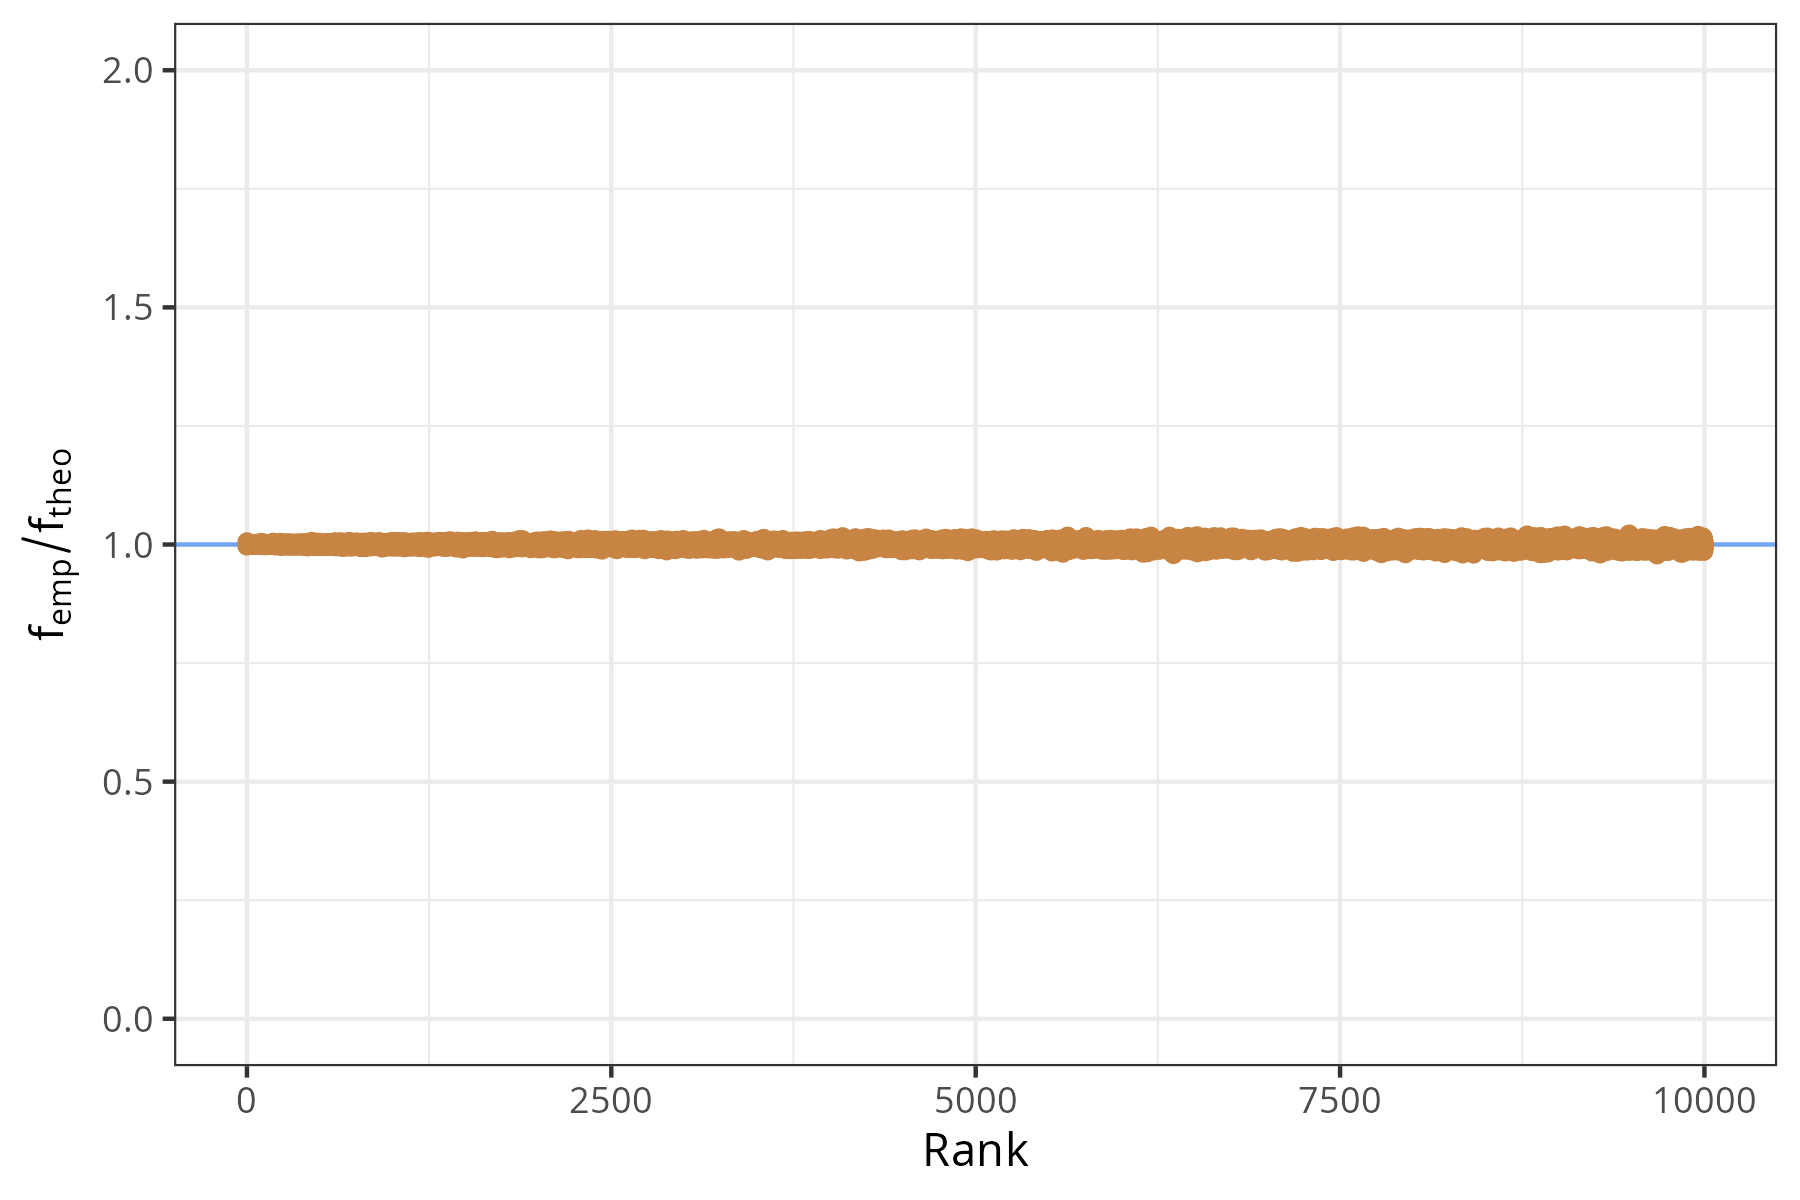
\includegraphics[width=\textwidth]{figures/ratio/sysbench.png}
        \caption{Sysbench}
    \end{subfigure}

    \vspace{1em} % Space between rows
    
    % Third row
    \begin{subfigure}{0.46\textwidth}
        \centering
        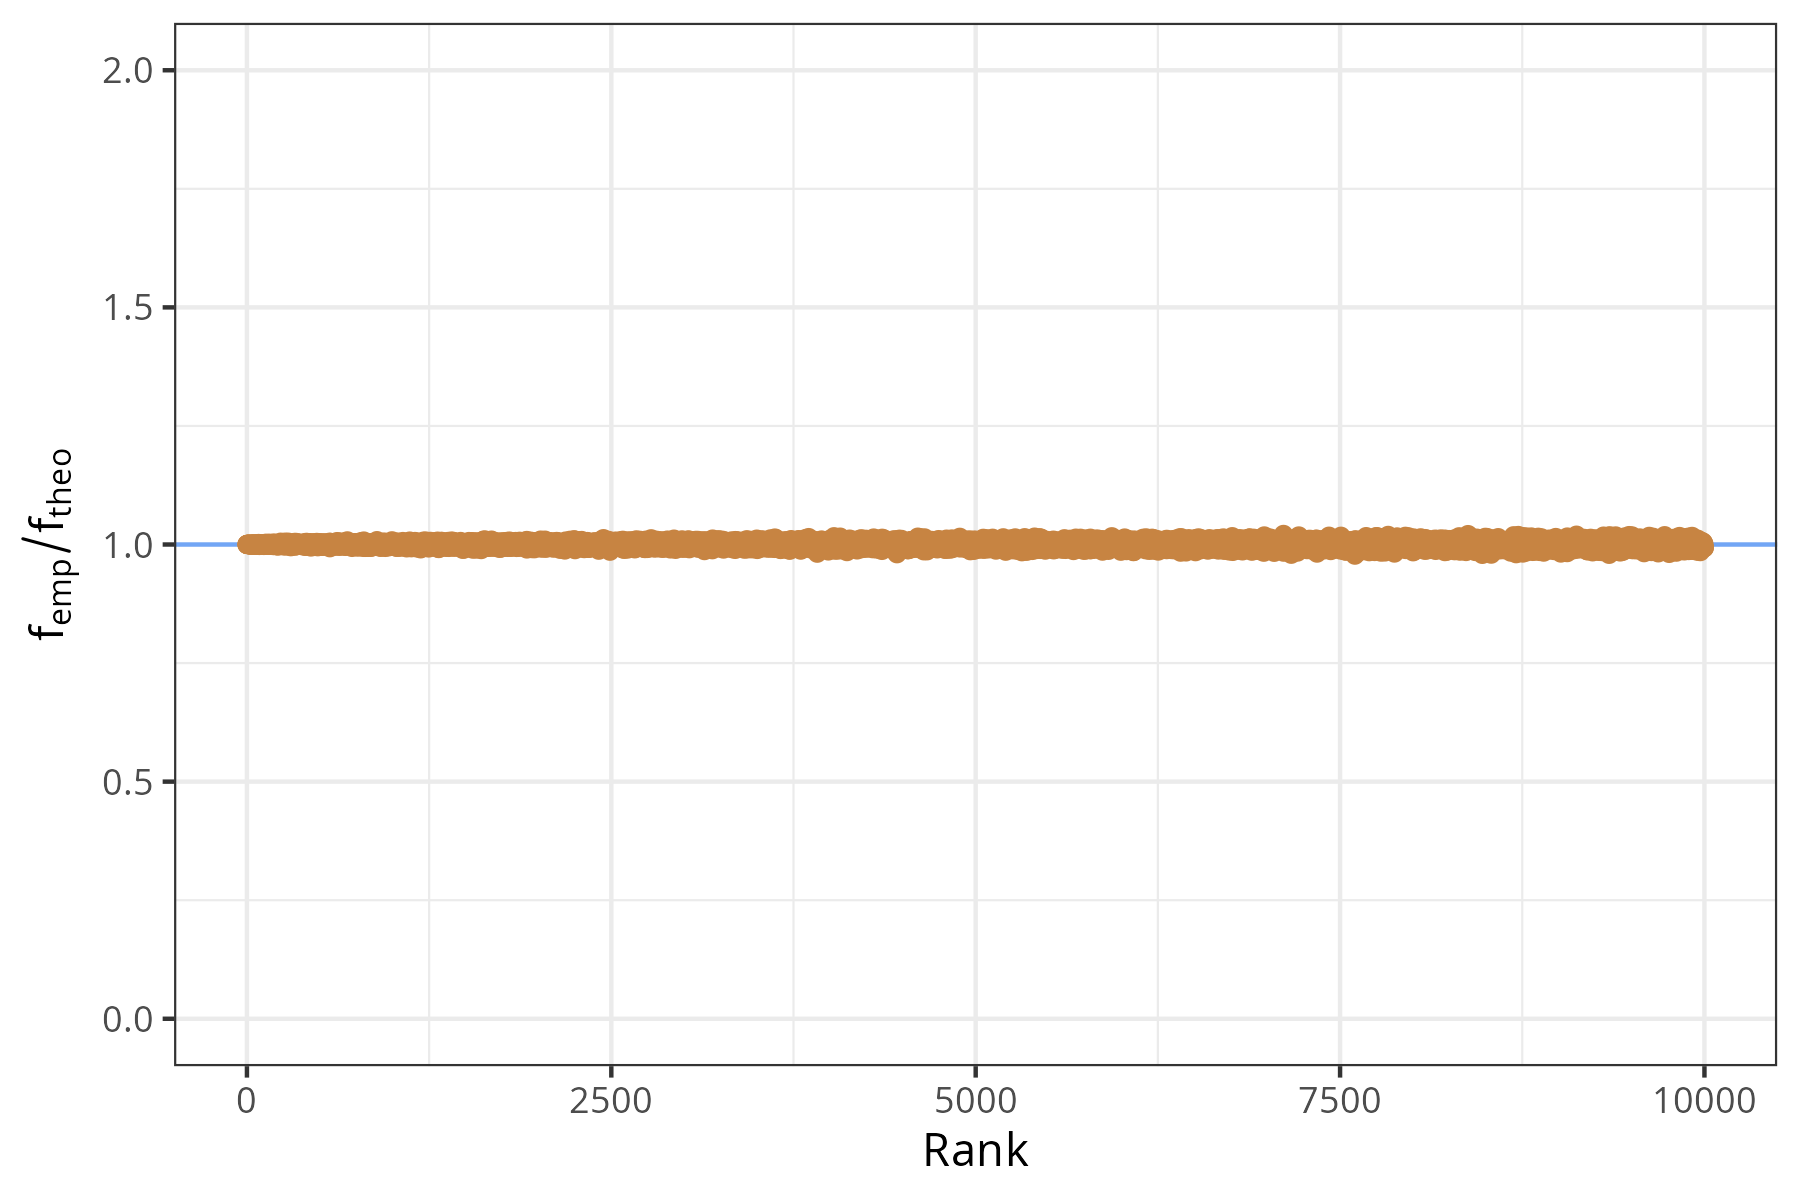
\includegraphics[width=\textwidth]{figures/ratio/marsaglia.png}
        \caption{Condensed Table Lookup}
    \end{subfigure}
    \hfill
    \begin{subfigure}{0.46\textwidth}
        \centering
        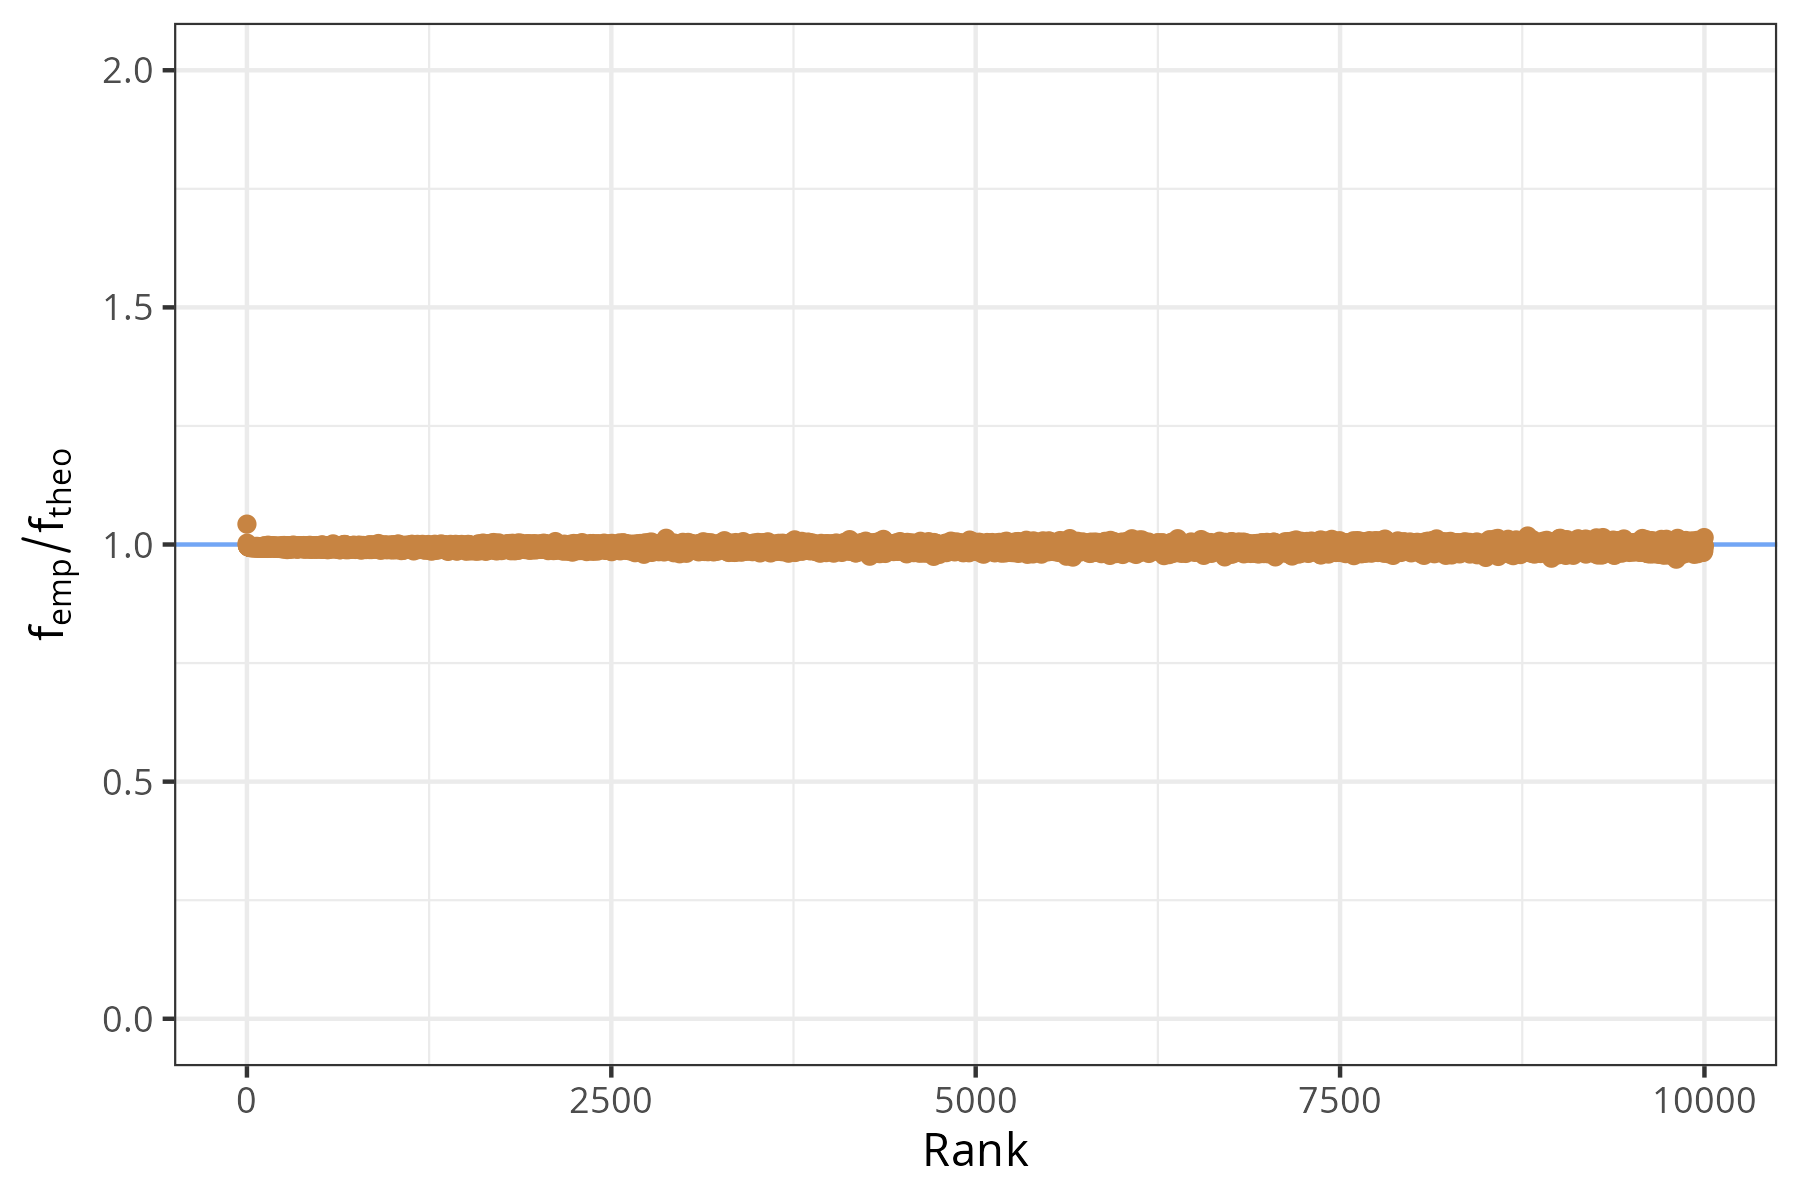
\includegraphics[width=\textwidth]{figures/ratio/rejection.png}
        \caption{Rejection}
    \end{subfigure}

    \caption{All distributions have support size $10^6$ and have $10^9$ samples}
    \label{fig:ratio-graphs}
\end{figure}